% !TEX root = ../master.tex
\chapter{Fundamentals}
\label{chap:sota}
In this chapter the state of the art of the technologies and concepts used in this thesis are outlined.
A broad overview over object detection using computer vision and the control of elevator systems is given.
This forms the basis to further explore the problem and find possible solutions in the chapters afterwards.

\section{Computer Vision}

The field of computer vision tries to establish methods and algorithms 
that extract useful information out of image data to be used by machines. 
The field has a broad range of applications and is influenced by various subjects such as methematics, physics and computer science.
Therefore \textcite{zhang2017imageprocessing} coined the term of \emph{image engineering} to localize the methods that deal with obtaining data from images. 
\textcite{zhang2017imageprocessing} defines three abstraction layers that these methods operate on (see figure \ref{fig:sota:imageengineering}).
\emph{Image processing} deals with the \enquote{manipulation of an image to produce another (improved) image} \autocite[][]{zhang2017imageprocessing}. 
It includes image capturing, representation and reconstruction.
\emph{Image analysis} is concerned with the extraction of higher level data from the image which described the objects and features present in the image.
To gain domain knowledge about the content of the image, this data can be processed by the means of \emph{image understanding}. 
This data can then be used to make decisions about the objects in the image.
Since the methods of each layer operate on data of the lower layer, a complex computer vision system employs methods from all three fields.  

\begin{figure}[hbt]
	\centering
	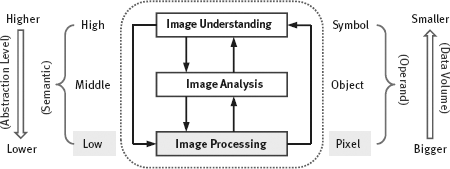
\includegraphics[width=0.8\textwidth, keepaspectratio]{08_Chapter01_fig1-4}
	\caption{\label{fig:sota:imageengineering} Levels of image engineering. 
	Reprinted from \textcite[][Chapter~1]{zhang2017imageprocessing}}
\end{figure}

\subsection{Image Representation}
Image data can be captured with different systems which produce image data of various dimensions.
It consists of information that can be visualized in any manner, such as still picture in color or grey-scale, a video, or a volumetric scan \autocite[][Chap.~1]{zhang2017imageprocessing}.
In general an image can be though of as a function $f: D \rightarrow V$, 
where $D$ is the domain of the location of an point in the image 
and $V$ is the domain of the properties of the real world represented at this point.
Typical examples for $ D $ are two dimensional images where the points are of the form $ (x, y) $, three dimensional images with points of the form $ (x, y, z) \in \mathbb{R}^3 $ or videos with points of the form $ (x, y, t) \in \mathbb{R}^3 $ where $ t $ is the time dimension.
Typical examples for $ V $ are grey-scale images where the luminosity is described as a value in $ \mathbb{R} $ or a colored image where the color is describes as a red-green-blue $ (r, g, b) \in \mathbb{R}^3 $.

For digital images $V$ and $D$ are discrete with upper and lower limits.
In two dimensions a image point a discrete position $ (y, x) \in \mathbb{N}^2 $ is called a \emph{pixel},
in three dimensions a point $ (x, y, z) \in \mathbb{N}^3 $ is called a \emph{voxel}.
In order to store such an image on a computer a \emph{matrix representation} can be chosen.
Examples:
For two dimensional images this matrix is element of $ V^{X \times Y} $, where $ X $ and $ Y $ describe the width and height of the image \autocite[][Chap.~1]{zhang2017imageprocessing}. For three dimension $ V^{X \times Y \times Z} $ can be used, where $X Y Z$ describe the length of the image in each spatial direction. 
A discrete (digital) two dimensional \ac{RGB} color image can be represented as a matrix  $ F \in \mathbb{N}^{X \times Y \times 3} $.
The value of a pixel can then be obtained using the function $ f_F: \mathbb{N}^2 \rightarrow \mathbb{N}^3 ; (x, y) \mapsto f(x,y) = F_{x,y} $.

\subsection{OpenCV Computer Vision Library}
OpenCV (Open Computer Vision Library) is a free (as in freedom) and open-source library,
which collects many common functionalities for advanced computer vision.
The \ac{BSD} license allows it to be used in private, academic and commercial contexts. 
It is written in performant C/C++ and offers \ac{API} bindings for C++, Python and Java on Windows, Linux, Mac OS, iOS and Android \autocite[][]{opencv2018opencv}.
It features algorithms that operate on all three layers of image engineering as defined by Zhang 
and can be used to implement complex visual systems. 
Its documentation is extensive and offers practical examples for a lot of problems it solves.



\subsection{2D Object Detection}

\subsubsection{Convolution Kernels}

A key concept in image processing is the application of an \emph{convolution matrix} to an image, which is also known as a \emph{kernel}. 
It is a small matrix with the same dimensions as the image it is applied to. 
For \ac{2D} images $ 3 \times 3 $ or $5 \times 5 $ kernels are used. 
To apply the kernel to the image, they are convoluted.
This is done for each pixel individually by \enquote{overlaying} the kernel with its center onto it. 
Then the sum of the element-wise multiplication of the kernel and the overlaid area of the image is calculated in order to determine the resulting pixel value in the output image.
For a \ac{2D} image $ F \in \mathbb{N}^{X \times Y} $ the convolution $ H \in \mathbb{N}^{X \times Y} $ using the kernel $ K \in \mathbb{N}^{M_i \times M_j} $ is calculated with the formula in figure \ref{eq:sota:convolution}:

\begin{figure}[h!]
\begin{equation*}
H_{x,y} = \sum_{i=0}^{M_i-1} \sum_{j=0}^{M_j-1} F_{x+1-a_i, x+j-a_j}K_{i,j}
\end{equation*}
\caption{Application of an 2D convolution kernel. Reprinted from the \textcite[][]{opencv2018kernel}}
\label{eq:sota:convolution}
\end{figure}

Convolution kernels can be used to find local features in an image or apply general local operation.
This includes blurring with the Gaussian filter, and edge detection with the Sobel filter in X and Y direction or with the Laplace filter (see figure \ref{eq:sota:kernels}).
It can also be used to sharpen an image. 

\begin{figure}[h!]
\begin{equation*}
    G = 
    \dfrac{1}{16}
    \begin{bmatrix}
    1 & 2 & 1 \\
    2 & 4 & 2 \\
    1 & 2 & 1
    \end{bmatrix}
    ;
    G_x = 
    \begin{bmatrix}
    1 & 0 & -1 \\
    2 & 0 & -2 \\
    1 & 0 & -1
    \end{bmatrix}
    ;
    G_y = 
    \begin{bmatrix}
    1 & 2 & 1 \\
    0 & 0 & 0 \\
    -1 & -2 & -1
    \end{bmatrix}
    ;
    D_{xy}^{2} = 
    \begin{bmatrix}
    1 & 1 & 1 \\
    1 & -8 & 1 \\
    1 & 1 & 1
    \end{bmatrix}
\end{equation*}
\caption{Examples for kernels left to rigth: Gaussian blur filter, Sobel filter in X direction, Sobel filter in Y direction, Laplace filter}
\label{eq:sota:kernels}
\end{figure}

\subsubsection{Background Subtraction}
Background subtraction used to detect areas of interest in a video.
Especially in a static camera setup, everything that moves can be considered the foreground and everything that stays static is the background. 
To do so, a model of the background without any moving objects is needed.
It acts as a reference frame to compare the current frame of a video against.

If an image is available, that only shows the background of a scene,
\emph{static background subtraction} can be used.
In this method, the current frame of the video and the background are blurred 
and the element-wise absolute difference between the images is calculated.
If the absolute difference for a pixel is higher than a specified threshold, then the pixel is considered part of the foreground.
This method uses the given background image as a static model for the background and does not update the model if the background changes.

When no pure background image is available 
or if the background can change over time, e.g. by different lighting,
the background model needs to be regularly adapted.
\textcite[][]{piccardi2004background} presents an overview of techniques used to create such a model, 
whereas here only a subset is presented:

\begin{itemize}
    
    \item \textbf{Running Gaussian average} For each pixel $ I $  in the grey-scale video image a running average $ \mu{}_t$ is calculated, that is updated in each frame by the formula $ \mu{}_t = \alpha{}I_t + (1 - \alpha)\mu{}_{t-1} $, where $ \alpha $ is an weight that determines how fast the model is updated. The variance $ \sigma{}_t $ is calculated similarly. A pixel $ I_t $ is considered foreground if $ |I_t - \mu{}_t| > k\sigma{}_t $ holds, where $ k $ is a parameter that determines the threshold sensitivity of the algorithm.
    \item \textbf{Mixture of Gaussians} Instead of assuming a single value likelihood distribution for each pixel, multiple Gaussian distributions are used in this method introduced \textcite[][]{stauffer1999background}. 
    When using $ K $ distributions this enables the distinction of $ K $ types of background and foreground, which improves the detection rate in outdoor scenes where e.g. leafs and branches of trees might be present. 
    For each of the $ K $ distributions the peak amplitude $ \omega{}_{i,t} $, average $ \mu{}_{i,t} $ and variance $ \sigma{}_{i,t} $ are stored.
    The distributions are ranked by the ratio $ \omega{}_{i,t} / \sigma{}_{i, t}$, since more narrow distributions are assumed to belong to a background classification.
    The distributions are checked in order of their rank to accept a pixel value when $ (I_t - \mu{}_{i,t})/\sigma{}_{i,t} > 2.5 $ holds.
    If $ \omega{}_{t} $ of the first accepting distribution is higher than a threshold, the pixel is considered background.
    The distribution parameters are updated using a running calculation (as above) when a new pixel value is a accepted by it.
    If no distribution accepts the value, the distribution with the lowest ranked is replaced by a new distribution centered around the new value with a high variance.
    Improved forms of this algorithm exist, like \autocite[][]{chan2011background}, and are currently used.
    
\end{itemize}

Since video images can contain pixel level noise, it is useful convert color video to grey-scale and to blur the images before applying the background subtraction.

\subsubsection{Blob Detection}

A \emph{blob} in a binary mask image is an area that consists of 

what is a blob

first explain contour (what are contours: outlines of connected areas in a binary mask) detection by border following \autocite[][]{suzuki1985border}



\autocite[][]{opencv2018blob}
operates on binary masked image
\begin{enumerate}
    \item Find the contours present in the image and calculate their centers
    \item Group these centers based on a threshold for the distance for their location
    \item From these groups, find overall center and estimate area and radius of the blob
\end{enumerate}

TODO

\subsubsection{Convex Hull}

TODO
edge detection, outline detection, silouettes, contours
foreground background mask from video image
background substraction
convex hull


\subsection{3D Volume Estimation}

TODO describe what is ment by this

\subsubsection{Camera Projection and Calibration}

Since camera lenses use a perspective projection to produce images, 
there are several considerations needed when working with \ac{3D} scenes that are captured.
The points in the 3D scene can be described as coordinates in the \emph{world space}.
In the perspective projection these points are seen from a single point in the camera, 
which is the sensor in a real camera.
To perform the projection the position of the point seen on the \emph{image plane} is calculated.
The image plane is the section of the scene that is seen by the camera in the distance of the focal length.
Figure \ref{fig:sota:camerprojection} shows how this projection can be visualized.
Note that the Z axis is pointing into the real world space in the direction the camera is looking to.
Since this projection is dependent on the focal length of the camera and the principal point, which is seen in the center of the image, it can be described as the intrinsic camera matrix $ A $ in the equation in figure \ref{eq:sota:camcalib}.
When world space and camera space coordinates are not the same, i.e. the camera is rotated or translated, there exists an additional rotation and translation matrix $ [R|t] $ that describes these external projection parameters.

\begin{figure}[hbt]
    \centering
    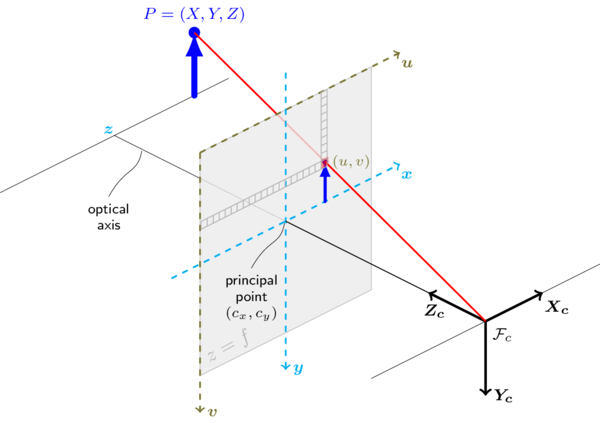
\includegraphics[width=0.8\textwidth, keepaspectratio]{opencv_pinhole_camera_model}
        \caption{Camera model to illustrate perspective projection of a 3D scene onto the image plane (grey). Reprinted from the \textcite{opencv2018calibration}}
    \label{fig:sota:camerprojection}
\end{figure}

\begin{figure}[h!]
\centering
\begin{equation*}
    s m' = A[R|t]M'
    \hspace{2em}
    \Longleftrightarrow{}
    \hspace{2em}
    s 
    \begin{bmatrix}
        u \\
        v \\
        1
    \end{bmatrix}
    =
    \begin{bmatrix}
        f_x & 0 & c_x \\
        0 & f_y & c_y \\
        0 & 0 & 1
    \end{bmatrix}
    \begin{bmatrix}
        r_{11} & r_{12} & r_{13} & t_1 \\
        r_{21} & r_{22} & r_{23} & t_2 \\
        r_{31} & r_{32} & r_{33} & t_3
    \end{bmatrix}
    \begin{bmatrix}
        X \\
        Y \\
        Z \\
        1
    \end{bmatrix}
\end{equation*}
\caption{Camera calibration with internal and external parameters. Reprinted from the \textcite{opencv2018calibration}}
\label{eq:sota:camcalib}
\end{figure}

The equation in figure \ref{eq:sota:camcalib} depicts how a point in the world coordinate system can be mapped to the image plane of a camera. 
The following list explains the mentioned coefficients:

\begin{samepage}
\begin{itemize}
    \item $ s $ is the scale factor for image, such that the z axis of the image plane is 1
    \item $ (X, Y, Z) $ is the 3D point in world space
    \item $ (u,v) $ is the projected point in the image plane
    \item $ A $ is the internal camera matrix
    \item $ (c_x, c_y) $ is the principle point in the world space seen at the image center
    \item $ f_x, f_y $ are the focal lengths in pixel units
    \item $ R $ is the external rotation matrix
    \item $ t $ is the external translation vector
\end{itemize}
\end{samepage}

The internal camera matrix $ A $ can be calculated from multiple images of an object with known structure and dimensions, called a \emph{calibration pattern} \textcite{opencv2018calibration}. 
For example an chessboard can be used, which is photographed from different positions and angles. 

The external parameter for rotation and translation can not be found from one camera alone.
In a multi-camera setup they can be found by triangulation of multiple points in multiple images that show the same scene from different angles.
If this triangulation is not possible because the points used for triangulation are not visible from all camera perspective, the rotation matrix an the translation vector can be found out by measuring the real world.
The rotation matrix can be calculated by measuring the relative rotation angles of the cameras to each other.
The equation in figure \ref{eq:sota:rotation} can be used to determine the combined rotation matrix when the rotation around the yaw, pitch and roll angles are known. 
Yaw pitch and roll describe the rotation around the Z, Y and X axis respectively.
The translation vector can be found by measuring the distance of the cameras to each other.

\begin{figure}[h!]
\centering
\begin{equation*}
    R
    =
    R_z(\alpha)R_y(\beta)R_x(\gamma)
    =
    \begin{bmatrix}
    cos \alpha{} & - sin \alpha{} & 0 \\
    sin \alpha{} & cos \alpha{} & 0 \\
    0 & 0 & 1 
    \end{bmatrix}
    \begin{bmatrix}
    cos \beta{} & 0 & sin \beta{} \\
    0 & 1 & 0 \\
    - sin \beta{} & 0 & cos \beta{}
    \end{bmatrix}
    \begin{bmatrix}
    1 & 0 & 0 \\
    0 & cos \gamma{} & - sin \gamma{} \\
    0 & sin \gamma{} & cos \gamma{} 
    \end{bmatrix}
\end{equation*}
\caption{External rotation matrix from rotation along the yaw, pitch and roll angles $ \alpha{} $ , $ \beta{} $ and $ \gamma{} $ }
\label{eq:sota:rotation}
\end{figure}

Furthermore real lenses introduce optical aberrations and 
there exists \emph{distortion} in camera images.
Distortion is visible in the effect where straight lines appear curved in the image representation.
There exists two kinds of distortion that can occur, namely radial and tangential distortion \autocite[][Fig.~2]{weng1992distortion}.
Radial distortion makes points appear closer together or further apart depending on their distance to the image center. 
It is visible as a \enquote{barrel} or \enquote{pillow} effect on rectangular lines. 
Tangential distortion causes a rotation of the image depending on the distance and angle of a point to the image center.
The amount and type of distortion is part of the internal camera parameters.
Just as the matrix of intrinsic parameters, the parameters for the distortion can be calculated from images of structures with known dimensions
\autocite{opencv2018calibration}.

\subsubsection{Single View Estimation}
When the geometric shape of an \ac{3D} object is roughly known beforehand and only its exact outline and scale varies, it is possible to estimate its volume from its outline in a single image.
The assumption here is that the volume scales with the area, that the object covers on the image \autocite{levine1989microwave} \autocite[][]{wang2017apple} \autocite[][]{sapkal2017volume} .
Therefore a reference object with known dimensions is necessary to calculate the scale against.
This approach avoids the need to multiple cameras and a \ac{3D} calibration
However it does notgeneralize to \ac{3D} objects of unknown shape.

\subsubsection{Feature Based Scene Reconstruction} 
stereo vision
of full \ac{3D} reconstruction of each point
TODO

key concept: photoconsistency : a voxel is photoconsitent when 



\begin{figure}[hbt]
	\centering
	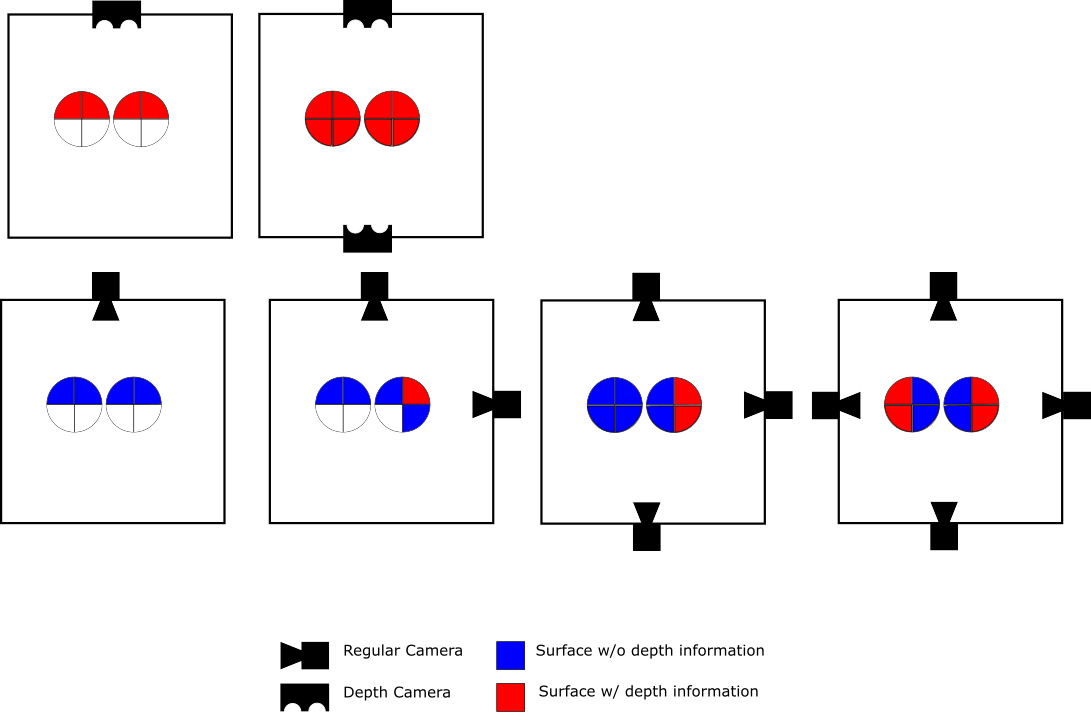
\includegraphics[width=1.0\textwidth, keepaspectratio]{resources/multiview}
	\caption{\label{fig:sota:mulitviewtop}Concept of depth reconstruction in a 2D multi-view situation.
	Adapted from \textcite[][]{sonaten2011volume}}
\end{figure}

\subsubsection{Silhouette Based Volume Reconstruction}

The \emph{silhouette} of an object within an image is intuitively defined 
as a binary mask describing the areas of the image in which the object is present. 
The edges of this areas describe the contours of the object.
The silhouette can be obtained by image segmentation of the original image \autocite[][Chap.~2]{zhang2017imageanalysis}.
Depending on the camera perspective different portions of the object are visible.
This can be used to reconstruct an image of $N+1$ spatial dimensions from images of $N$ spatial dimensions.



shape from silhouette creates visual hull (no concavities)
\autocite[][]{laurentini1994hull}

TODO
Volume Intersection (photoconsitency is given with an additive approach that uses polyhederons and backrpojection to generate intersection cones)
\autocite[][]{}

simple voxel substraction by removing all voxels that are not in all silhouetts

Space Carving (substractive technique that begins with a full voxel scene. the surface oof the scene is carved away pixel per pixel untill all surface voxels  are photoconsistent)
\autocite[][]{kutulakos1999spacecarving}

TODO
single view, multiview, depth sensors
estimation by pixel area
interpolation of depth information by combinding views
bounding / section box
convex hull in 3d by mask
Space Carving with silhouettes
simple voxel substraction method
visual hull 



\begin{figure}[hbt]
	\centering
	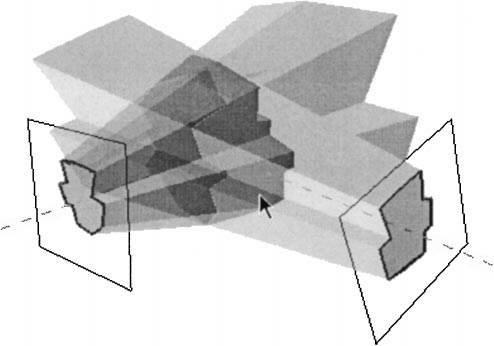
\includegraphics[width=0.6\textwidth, keepaspectratio]{resources/volume_intersection_bottino}
	\caption{\label{fig:sota:volumeintersection} Volume intersection of cones from silhouettes.
	Reprinted from \textcite[][]{bottino2001silhouette}}
\end{figure}

\section{Elevator Control}

When looking at elevator systems that are installed in buildings
one property that is noticeable to the passenger, except for the physical properties, is the way the elevators are moved in order to pick up and deliver the passengers to their destination.
The algorithms used to control this movement influence how long the passenger needs to wait for a cabin and how long their journey takes.
Therefore it affects the perceived quality of the system.
However in buildings with an increased traffic demand, it is necessary to use elevator systems with multiple cabins and more complex control strategies.
In this section the general principles about those control strategies are laid out.

\subsection{System Components}

In order to gain an understanding of how an elevator system is controlled,
it is useful to look at the components a general system includes.
To do so, the mechanisms involved in a typical elevator ride 
from a passenger perspective shall be outlined.
Figure \ref{fig:sota:systemcomponents} gives an general overview over the involved logical components and their connections.

\begin{figure}[hbt]
	\centering
	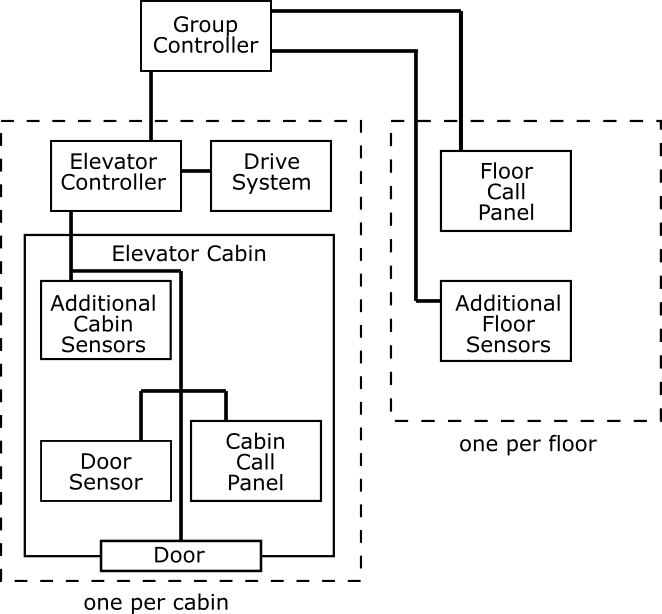
\includegraphics[width=0.8\textwidth, keepaspectratio]{resources/systemcomponets}
	\caption{\label{fig:sota:systemcomponents} General components of an elevator control system. Adapted from \textcite[][pp.~4,16]{xang2016trafficlist} and  \textcite[][p.~10]{siikonen1997models}}
\end{figure}

When a passenger wants to take the elevator from one floor to another,
they press a button on the \emph{floor call panel} and issue a \emph{hall call} (or \emph{reservation call}, \emph{landing call}) to the system \autocite[][pp.~6--10]{siikonen1997models}.
This hall call signals to the system that an elevator needs to pick them up.
The button pressed might be a simple push button, but can also be more complex 
and capture information about the direction or destination of travel \autocite[][pp.~89--93]{unger2015aufzuege}.
Even before the passenger presses the panel button, \emph{additional sensors} 
on the floor can detect their intent to use the elevator and gather more information about them.
This can include among others camera systems \autocite[][]{lin2011control}, badge scanners, or \enquote{smart home} installations \autocite[][]{kwon2014sensor}.
In a multi-elevator system the hall call is registered by the \emph{group controller} and stays active until it is deleted when an cabin picks up the passenger.
The group controller \emph{schedules and dispatches} an elevator move to the respective floor and serve the call.
In case of a single-elevator system no group controller is necessary.
Different scheduling algorithms can be used to determine which cabin should serve which hall call next.
The dispatch signal is picked up by the \emph{elevator controller} of the respective cabin, which then instructs the \emph{drive} system to move the elevator along the shaft to the respective floor by actuating the motors.

Once a cabin stops at the floor, it opens its \emph{door} and the passenger enter the elevator.
To select their destination floor, they use the \emph{cabin call panel}.
This \emph{car call} (or \emph{destination call}) \autocite[][pp.~6--10]{siikonen1997models} is passed to the group controller, 
which schedules the elevator to move to the destination floor at some time.
The group controller needs therefore to consider hall calls, as well as car calls in its scheduling algorithm
Before the elevator starts to move, the door closes again, if no obstacle is detected by the \emph{door sensor}.
Until the elevator serves the destination floor, the car call stays active.
\emph{Additional sensors} inside the cabin provide more information about the passengers inside.
This can include among others a weight scale to measure the total weight utilization, or a kind of camera system \autocite[][]{xang2016trafficlist}.
Further more the position of each elevator is known to the group controller.

\subsection{System Classifications}

Elevator systems come in different configurations with different purposes.
Depending on their use cases different technical implementations can chosen.
Therefore they can be classified in various dimensions.

The first observation to make is the \textbf{number of shafts and cabins} in the system.
The main difference comes in the scheduling complexity regarding single-cabin versus multi-cabin systems.
Systems with multiple elevators need a group controller to decide which cabin serves which hall call.
This decision can be non-trivial as laid out in section \vref{sec:sota:strategies}.
When only one cabin is used, the scheduling becomes more straightforward.
In small residential buildings an single cabin might be sufficient.
However in buildings with larger passenger amounts, such as office buildings, a multi-elevator setup can become necessary increase the handling capacity.

Next is the classification by the \textbf{type of objects or people} that are transported in the system. Especially important is the distinction of the purpose of the elevator system regarding whether people and / or large objects can be conveyed.
\textcite[][pp.~141--158]{unger2015aufzuege} describes the properties of the most common types:

\begin{itemize}
    \item Cabins that carry \textbf{only people} 
    typically have a premium interior decoration, such as glass, mirrors or stainless steel.
    Usually also cargo can be transported, but large goods might damage the cabin.
    Examples for a building that uses such elevators are office buildings, residential buildings or hotels.
    
    \item Elevators for \textbf{large cargo and people} 
    have a more simple interior that is more resistant to damage by lifting carts. 
    However security measures regarding the doors are taken, such that the elevator is also safe to use by people. 
    Typically a high payload weight and dimension can be moved.
    Examples for the usage of this type are factories, storage buildings or hospitals. 
    
    \item Lifts that carry \textbf{only small cargo} can be found for example in restaurant kitchens to transport dishes.
    The cabin is not used by people and the system is controlled purely from outside call panels. 
    Due to the size restriction only a smaller weight needs to be transported.
    
    \item Cabins that convey \textbf{only large cargo} but no people can only be controlled from the outside call panel and have fewer safety restrictions, even though the cabin can be entered for loading and unloading. 
\end{itemize}

This excerpt of the list is far from complete and \textcite[][pp.~141--158]{unger2015aufzuege} lists even more types, 
such as lifts for wheel chairs, the never-stopping paternoster or elevators on construction sites.
However these are not in the scope of this thesis and are not further considered.

Another interesting distinction to consider is the \textbf{amount of floors} that is served by an elevator system.
The amount of floors influences the heeded handling capacity of the system.
The more floors there are, the more people need to travel a potentially longer distance.
While a building with only a few floors can be handled by a single elevator,
buildings with up to 40 stories require the use of elevator groups.
When more than 40 floors need to be served, 
introducing a \emph{sky lobby} can be beneficial, 
where a fast shuttle transports passengers between the main lobby and the sky lobby. Passengers can then switch the elevator to reach their final destination \autocite[][p.~9]{hakonen2003simulation}.

%
%TODO
%- by type of sensory to haul the car
%-- single button
%-- direction button
%-- destination control
%-- camera system

%TODO additional travel information: how many people inside and outside, up / down / floor %select inside / outside, everyone presses?, video? 
%destination control system


\subsection{Passenger Traffic Patterns}
Passenger traffic patterns are typical streams of passengers going from one floor to another.
Those patterns are reoccurring regularly based on the time of the day.
The movement of passengers can be described with three directions: \emph{incoming}, \emph{outgoing}, and \emph{inter-floor} traffic.
With those directions the traffic patterns can be described, as they focus on one of the directions, but also incorporates components of passengers heading in other directions \autocite[][p.~259]{siikonen1993simulation}.
According to multiple sources, three general patterns are present in office buildings \autocite[][pp.~1--2]{beers2015arrivals}
\autocite[][pp.~6--7]{axelsson2013strategies}
\autocite[][p.~194]{unger2015aufzuege}
\autocite[][p.~14]{siikonen1997models}:

\begin{itemize}
    \item \textbf{Up-peak traffic} In the morning the majority of passengers in an office building constitutes to an incoming traffic.
    They arrive at the entrance lobby and travel to different upper floors to fill the building.
    The lift cars potentially need to stop at every level and return to the lobby without passengers to pick up new ones. 
    This reduces the utilized capacity and puts a high load on the elevator system to convoy all passengers in time.
    \item \textbf{Down-peak traffic} In the evening the majority of the passengers are leaving the office building and travel from arbitrary upper floors to the main lobby.
    Most of the passengers constitute to outgoing traffic.
    The elevator system needs to pick up passengers at every level. 
    Reverse to the up-peak traffic, the cars are empty when returning from the lobby.
    Similar to the up-peak traffic this situation induces a high stress on the system.
    \item \textbf{Inter-floor traffic} All other traffic that is neither incoming nor outgoing can be considered inter-floor traffic. Passengers that travel from one floor to another but are not entering or leaving the building are the majority in this situation.
\end{itemize}

\begin{figure}[hbt]
	\centering
	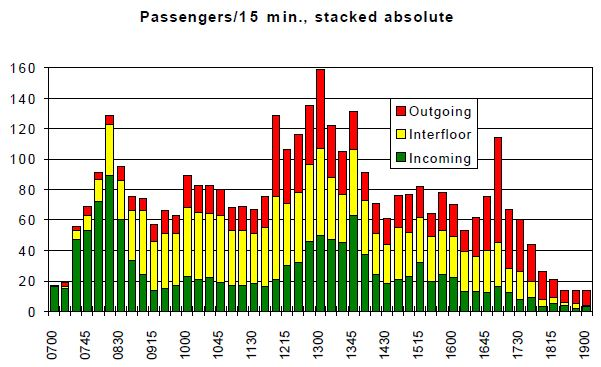
\includegraphics[width=0.8\textwidth, keepaspectratio]{resources/traffictimes}
	\caption{\label{fig:sota:traffictimes} Exemplary traffic component profile for an office building.
	Reprinted from \textcite[][p.~14]{siikonen1997models}}
\end{figure}

%Figure \ref{fig:sota:trafficpatterns} depicts the former mentioned traffic components.
Figure \ref{fig:sota:traffictimes} shows an example of how the traffic components contribute to overall traffic in an office building. A clear peak of incoming traffic in the morning and outgoing traffic in the evening are visible.
This information can be used to model simulations and predict traffic in various circumstances.
It has significant impact on the scheduling principles employed for each situation in order to improve the efficiency of an elevator system.

%\begin{figure}[hbt]
%	\centering
%	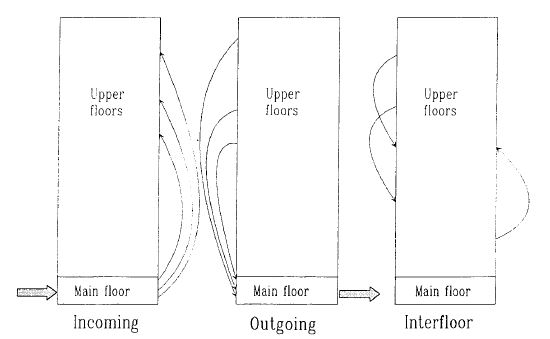
\includegraphics[width=0.8\textwidth, keepaspectratio]{resources/trafficpatterns}
%	\caption[]{\label{fig:sota:trafficpatterns} Typical categories of passenger traffic: Incoming, Outgoing and Inter-floor.
%	Reprinted from \textcite[][p.~259]{siikonen1993simulation}}
%\end{figure}

% TODO or use \textcite[][p.~12]{sorsa2005destination} as broader image 

\subsection{Control Strategies}
\label{sec:sota:strategies}

Elevator control strategies deal with the assignment of hall calls and car calls to elevator rides in order to derive a stopping schedule for the cabins in the system.
The way this schedule is set up affects
the performances regarding the criteria laid out in section \label{sota:sec:perf}.
An appropriate control algorithm must be chosen in order to optimize for performance criteria
depending on the type of elevator system, it's use purpose and the current passenger traffic.
Depending on the type of elevator system different control strategies are used, some of which are listed below.

\subsubsection{Sequential Control}
In contrast to the strategies below, 
this strategy is only applicable to a single-lift system.
The system answers hall calls in the order they arrive 
and executes the car call with priority before moving on to serve the next hall call.
This way only one ride is performed a time and the calls are executed in sequence. This method is also called \emph{single call automatic control} or \emph{non-collective control}.
Drawbacks of this strategy are a increased passenger waiting time and an decreased handling capacity.
However for cargo lifts, this can beneficial if only on cargo item can fit the cabin at a time
\autocite[][p.~238]{barney2016handbook}.

\subsubsection{Collective Control}
This is the \enquote{most common form of automatic control} \autocite[][p.~237]{barney2016handbook}.
Hall calls are answered in the order of the floors they originate from rather than their temporal order.
On the way up and down the cabin collects all the hall calls and deliver car calls also following the floor order.
Different variations of this approach are available, where the direction of the hall call is ignored, only downward calls are collected only upwards calls are collected, or the call direction is considered for collection in both directions.
This approach can be expended to a elevator system with group control, such that a hall call is answered by the first cabin to pass the floor in the desired direction \autocite[][p.~238]{barney2016handbook}.
When all cabins are idle, the nearest available is assigned to a call. Hence this strategy is also called \emph{nearest car}
\autocite[][p.~244]{barney2016handbook}.

\subsubsection{Zone Approach}
In this approach the floors of the building are divided into static, continuous zones also called \emph{sectors} \autocite[][p.~247]{barney2016handbook}. 
Typically there are is one zone per elevator in the group. 
Each lift in the group serves hall calls from only one sector
while also delivering passengers to floors outside of this zone
\autocite[][pp.~3--6]{axelsson2013strategies}.
The order of serving of the hall calls is based on the collective control.
A lift is currently outside of its zone, 
the zone can be served by lifts from sectors above and below it.

The distribution of zones can be chosen based by the amount of passengers on each floor.
This approach is useful when the traffic is evenly distributed across the building, such as in interfloor traffic. It can be complemented with controls for special condition to react to peak-traffic \autocite[][p.~247]{barney2016handbook}.
The static zone approach can be extended to a dynamic sector approach where the sectors are not limited by static floor numbers but by the position of the elevators \autocite[][p.~250]{barney2016handbook}.

\subsubsection{Cost-function based approches}

\subsubsection{Parking Policies}

TODO
single elevator  vs multi elevator
TODO: more types

\autocite[][pp.~3--4,10]{beers2015arrivals}
- parking polcies
- call allocation

\autocite[][pp.~3--6]{axelsson2013strategies}
- search based
- rule based
- genetic algorithm




\subsection{Performance Criteria}
\label{sota:sec:perf}

In order to evaluate the performance of an elevator system some metrics about it are commonly considered.
They are used to check if a planned system fulfills the requirements that the expected traffic poses. 
The metrics are mostly perceived as part of the service quality by the passengers.
Many of them are linked together and influence each other.

% General cite:
%\autocite[][p.~10]{beers2015arrivals}
%\autocite[][p.~7]{hakonen2003simulation}
%\autocite[][pp.8-9]{siikonen1997models}
%\autocite[][p.~194]{unger2015aufzuege}

\begin{itemize}

    \item The \textbf{passenger waiting time} 
        describes the amount of time between the arrival of a passenger at the landing floor 
        and their entry into the elevator cabin 
        \autocite[][p.~7]{hakonen2003simulation}\autocite[][pp.8-9]{siikonen1997models}.
        
    \item The \textbf{passenger ride time} 
        measures the time between the entering of a passenger into the cabin 
        and them exiting the cabin on the destination floor
    \autocite[][pp.8-9]{siikonen1997models}.
    
    \item The \textbf{total journey time}, 
        also called \emph{total service time} \autocite[][p.~10]{beers2015arrivals} or \emph{time to destination},
        describes the total time a passenger spends in the system 
        and is calculated by the sum of waiting and ride time
        \autocite[][pp.8-9]{siikonen1997models}.
        
    \item The \textbf{round trip time} 
        describes the time it takes for a single elevator to collect passengers at the lobby,
        deliver them to the upper floors and return to the lobby. 
        This measure is critical in the up-peak traffic
        \autocite[][pp.8-9]{siikonen1997models}.
        
    \item The \textbf{handling capacity}, 
        also called \emph{5-minute interval}
        \autocite[][p.~194]{unger2015aufzuege},
        describes the maximum number of passengers that can be transported (into the upper most floor) during up-peak traffic
        \autocite[][pp.8-9]{siikonen1997models}.
        It is dependent on the round trip time.
        In theoretical considerations a maximum utilization of 60-80\% of the capacity is used for this scenario
        \autocite[][p.~194]{unger2015aufzuege}\autocite[][p.~7]{hakonen2003simulation}.
    
    \item The \textbf{interval time} 
        describes the time between departures of any cabin from the lobby 
        and influences the time a passenger hat to wait at the lobby
        \autocite[][pp.8-9]{siikonen1997models}.
    
    \item The \textbf{hall call time} 
        describes the time between the issuing of an hall call by a passenger and the cancellation of the call. 
        The call is canceled when an elevator is scheduled to serve the call floor and hence decelerates to stop at the floor
        \autocite[][pp.8-9]{siikonen1997models}. 
    
    \item The number of \textbf{total stops}
        necessary to serve an specified amount of passengers (or within a given time frame) is an indicator for the efficiency of the scheduling algorithm
        \autocite[][p.~194]{unger2015aufzuege}.
    
    \item The \textbf{energy consumption} 
        per ride or per time interval is an measure of economic interest. 
        However it does not influence the perceived service quality.
    
    \item The \textbf{capacity utilization} 
        of the cabins in spacial and weight dimensions is an interesting metric to observe, 
        since usually only 60-80\% of the capacity is used at a time 
        \autocite[][p.~194]{unger2015aufzuege}
        \autocite[][p.~7]{hakonen2003simulation}.
        This utilization can be even lower when large objects are present.
        The average utilization is further influenced by empty rides.
        
\end{itemize}

For each of the metrics it is common to calculate statistical figures, such as average, mean, minimum, maximum and standard deviation, which also can differ depending on the traffic situation.
These calculations can be based on theoretical consideration about the physical parameters of the system \autocite[][p.~194]{unger2015aufzuege}, simulations or heuristical observations in real buildings.
 
When the group controller schedules the elevators in a system, the order of dispatches influences the metrics listed above.
The elevator allocations are calculated by optimization of a cost function which takes the metrics in consideration.
Usually the waiting time is optimized, but also the ride time can be optimized in order to increase the handling capacity. \autocite[][p.~10]{siikonen1997models} 

\subsection{Optimization Approaches by Simulation}
TODO
model building etc: here is a lot of research in the topic utilizing theoretical multivariable model optimization, simulational approaches and heuristical approaches in real world (refs?)

\autocite[][pp.~7--11]{beers2015arrivals}
\autocite[][p.~193]{unger2015aufzuege}


TODO
